\documentclass[12pt]{article}

\usepackage[utf8]{inputenc}
\usepackage{float}
\usepackage{amsmath}
\usepackage{tkz-euclide}


\usepackage[hmargin=3cm,vmargin=6.0cm]{geometry}
%\topmargin=0cm
\topmargin=-2cm
\addtolength{\textheight}{6.5cm}
\addtolength{\textwidth}{2.0cm}
%\setlength{\leftmargin}{-5cm}
\setlength{\oddsidemargin}{0.0cm}
\setlength{\evensidemargin}{0.0cm}

%misc libraries goes here



\begin{document}
	
	\section*{Student Information } 
	%Write your full name and id number between the colon and newline
	%Put one empty space character after colon and before newline
	Full Name : Melis Ece ÜNSAL \\
	Id Number :  2237865\\
	
	% Write your answers below the section tags
	\section*{Answer 1}
	\subsection*{a)} Let $P_n$ be the string with  n 1's.\\
	$P_0 \rightarrow 0 0 0 0 0 0 0 0 0 \rightarrow 1 way$\\
	$P_1 \rightarrow \underline{1 0} \ 0 0 0 0 0 0 0 \rightarrow \dfrac{8!}{7!}=8 way$\\
	$P_2 \rightarrow \underline{1 0} \ \underline{1 0} \ 0 0 0 0 0 \rightarrow \dfrac{7!}{5!.2!}=21 way$\\
	$P_3 \rightarrow \underline{1 0} \ \underline{1 0} \  \underline{1 0} \ 0 0 0 \rightarrow \dfrac{6!}{3!.3!}=20 ways$\\
	$P_4 \rightarrow \underline{1 0} \ \underline{1 0} \  \underline{1 0} \ \  \underline{1 0} \ 0 \rightarrow \dfrac{5!}{4!}=5 ways$\\
	There cannot be more than 4 1's.Hence the result is 1+8+21+20+5=55.
	\subsection*{b)}
	Let $B_n$ be the string with  n 1's.\\
	$B_8 \rightarrow 1 \ 1 \ 1 \ 1 \ 1 \ 1 \ 1 \ 1 \ 0 \ 0 \rightarrow \dfrac{10!}{8!.2!} =45 $\\
	$B_9 \rightarrow 1 \ 1 \ 1 \ 1 \ 1 \ 1 \ 1 \ 1 \ 1 \ 0 \rightarrow \dfrac{10!}{9!.1!} =10 $\\
	$B_10 \rightarrow 1 \ 1 \ 1 \ 1 \ 1 \ 1 \ 1 \ 1 \ 1 \ 1 \rightarrow \dfrac{10!}{10!} =1 $\\
	Hence the result is 45 + 10 +1 =56.
	\subsection*{c)}
	From the Theorem 1 from the textbook(8.6) :\\ $n^m -C(n,1)(n-1)^m+....+(-1)^{n-1}C(n,n-1).1^m$\\
	=$3^4-C(3,1)2^4+C(3,2)1^3$=36.
	\subsection*{d)}
	
	\section*{Answer 2}
	
	
	\subsection*{a)} 
	Let's say a subset A of $a_n$ that does not contain consecutive numbers.We can divide A into two groups.\\
	Group 1 contains the element n,Group 2 does not contain n.\\
	We first get an expression for the number of Group 1,where n$\geq$2.Such a subset cannot contain n-1 due to constraint.So, any Group 1 subset can be obtained by adding n to a non-consecutive subset of $a_{n-2}.$\\
	Now we obtain an expression for the number of subset of Group 2 of $a_n$.Such a subset is a subset of $a_{n-1}$.\\
	A non-consecutive subset of $a_n$ is either of Group 1 or of Group 2.So the number of appropriate subsets of $a_n$ is \\
	\hspace*{3cm}	$ a_n = a_{n-2} +a_{n-1} $ for $n\geq2$.\\
	The initial conditions are $a_1=2$,because all of the subsets of this are non-consecutive and it is $2^1$ from $2^n$; and $a_2=3$ because it has just 1 consecutive subset which is itself so it is $2^2-1$ from $2^n-1$.
	\subsection*{b)} 
	$a_1=2$\\
	$a_2=3$\\
	$a_n= a_{n-1}+a_{n-2}$\\
	Let f(x) = $\sum_{n=0}^{\infty} a_nx^n$ \\
	
	$\sum_{n=3}^{\infty} a_nx^n = \sum_{n=3}^{\infty} (a_{n-1}+a_{n-2})x^n $\\  \\
	$\sum_{n=3}^{\infty} a_nx^n=\sum_{n=3}^{\infty} a_{n-1}x^n + \sum_{n=3}^{\infty} a_{n-2}x^n $\\
	
	$ \underbrace{ \sum_{n=3}^{\infty} a_nx^n}_{f(x)-a_1x-a_2x^2 } = \underbrace{\sum_{n=3}^{\infty} a_{n-1}x^n}_{x \sum_{n=3}^{\infty} a_{n-1}x^{n-1}} +  \underbrace{ \sum_{n=3}^{\infty} a_{n-2}x^n}_{x^2 \sum_{n=3}^{\infty} a_{n-2}x^{n-2}} $\\ \\
	\hspace*{1cm} $\downarrow \hspace{3cm} \downarrow \hspace{3cm} \downarrow $\\
	\hspace*{0.5cm} $ f(x)-2x-3x^2 = x(f(x)-2x) + x^2f(x)$\\
	\hspace*{0.5cm} $ = -x^2-2x = f(x)(x^2+x-1)$\\
	\hspace*{0.5cm} $ = f(x)=\dfrac{-x^2-2x}{(x^2+x-1)}$\\
	
	
	\section*{Answer 3}
	Theorem 1 from the textbook(8.2) can be used to solve this problem.The characteristic equation of the recurrence relation is $ r^{3} = 4r^2 + r -4.$It's root's are r=4,r=1,r=-1.Hence, the sequence $a_{n}$ is a solution to the recurrence relation if and only if \\
	\hspace*{3cm}	$ a_n = \alpha_1 4^n + \alpha_2 1^n+\alpha_3 (-1)^n$ for some constants $\alpha_1 ,\alpha_2,\alpha_3$.\\
	From the initial conditions,it follows that \\
	\hspace*{3cm} $a_0=4=\alpha_1 +\alpha_2+\alpha_3$\\
	\hspace*{3cm} $a_1=8=4\alpha_1 +\alpha_2-\alpha_3$\\
	\hspace*{3cm} $a_3=34=16\alpha_1 +\alpha_2+\alpha_3$\\
	Solving these equations shows that  $\alpha_1=2 ,\alpha_2=1$ and $\alpha_3=1$.Hence we conculude that\\
	\hspace*{3cm}	$ a_n = 2.4^n +  1^n+ (-1)^n$ 
	\section*{Answer 4}
	\underline{Definition:}An equivalence relation on a set X is a binary relation on X which is
	reflexive, symmetric and transitive.\\
	We check whether R is equivalence relation as follows:\\ \\
	\hspace*{2cm} (a) (\textit{Reflexivity}): ($x_1,y_1$)R($x_1,y_1$) hence $3x_1-2y_1=3x_1-2y_1$\\ \\
	\hspace*{2cm} (a) (\textit{Symmetry}): If $3x_1-2y_1=3x_2-2y_2$ then $3x_2-2y_2=3x_1-2y_1$.Hence ($x_2,y_2$)R($x_1,y_1$) \\ \\
	\hspace*{2cm} (a) (\textit{Transitivity}):If $(x_1,y_1)R(x_2,y_2)$ and $ (x_2,y_2)R(x_3,y_3)$ then $3x_1-2y_1=3x_2-2y_2$ and $3x_2-2y_2=3x_3-2y_3.$Since both of them equal $3x_2-2y_2$, $3x_1-2y_1=3x_3-2y_3$.Hence $ (x_1,y_1)R(x_3,y_3)$.\\ \\
	Consequently R is equivalence.\\ \\
	Now,first we need to find $(x_1,y_1)R(2,3) \rightarrow 3x_1-y_1=3*2-2*3=0 \rightarrow 3x_1-2y_1=0$.This is equivalent class for (2,3).\\
	After this we need to find equivalent class for (2,-3): $(x_1,y_1)R(2,-3) \rightarrow 3x_1-y_1=3*2-2*(-3)=12 \rightarrow 3x_1-2y_1=12$
	
	
	\begin{figure}[h]
		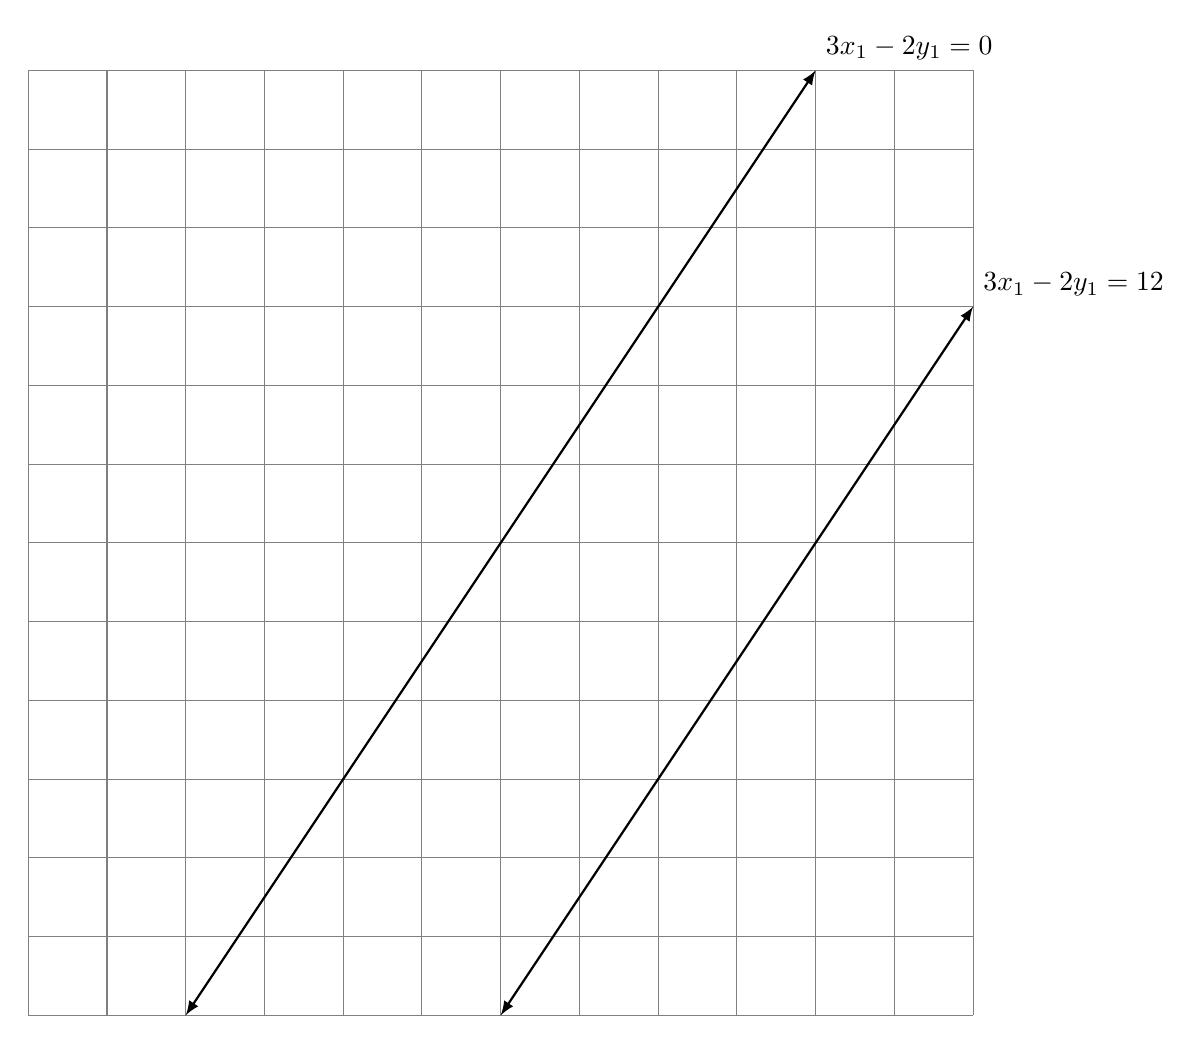
\begin{tikzpicture}
		\tkzInit[xmax=6,ymax=6,xmin=-6,ymin=-6]
		\tkzGrid
		\tkzAxeXY
		\draw[ thick,latex-latex] (-4,-6) -- (4,6) node[anchor=south west] {$3x_1-2y_1=0$}; % two points for drawing 2x+y=2
		\draw[ thick,latex-latex] (0,-6) -- (6,3) node[anchor=south west] {$3x_1-2y_1=12$}; % two points for drawing 2x+y=2
		
		\end{tikzpicture}
	\end{figure}
	
	
	
	
\end{document}